\documentclass[a4paper]{article}
\usepackage{import}
\usepackage{graphicx}
\usepackage{float}
\usepackage{pgfplots}
\usepackage{listings}
\usepackage{enumitem}
\usepackage{textcomp}
\usepackage{tikz}
\usetikzlibrary{decorations.pathreplacing} % for angle arc
\usetikzlibrary{angles, quotes, calc, positioning, trees} % for drawing angles
\pgfplotsset{compat=1.18,width=10cm}
\usepackage{tikz-cd}
\usepackage{booktabs}
\usepackage{cancel}
\usepackage{amsmath}
\usepackage{minted}
\usepackage{csquotes}
\usepackage{gensymb}
\usepackage{forest}
\usepackage{amsthm}
\usepackage{amssymb}
\usepackage{fontawesome} 
\usepackage{varwidth}
\usepackage{pgfplots}
\usepackage{lipsum}
\usepackage{mdframed} 
\usepackage{color}   
\usepackage{hyperref}
\newmdtheoremenv{theo}{Theorem}
\usepackage{mathtools}
\DeclarePairedDelimiter\ceil{\lceil}{\rceil}
\DeclarePairedDelimiter\floor{\lfloor}{\rfloor}

\hypersetup{
    colorlinks=true, %set true if you want colored links
    linktoc=all,     %set to all if you want both sections and subsections linked
    linkcolor=black,  %choose some color if you want links to stand out
}

% Define theorem styles
\newtheorem{theorem}{Theorem}[section]    % Theorems numbered within sections
\newtheorem{lemma}[theorem]{Lemma}        % Lemmas use the same counter as theorems
\newtheorem{corollary}[theorem]{Corollary} % Corollaries use the same counter as theorems
\newtheorem{proposition}[theorem]{Proposition} % Proposition uses the same counter
\newtheorem{property}[theorem]{Property}
\theoremstyle{definition}
\newtheorem{definition}[theorem]{Definition} % Now uses the same counter as theorems


% Remark-style theorem
\theoremstyle{remark}
\newtheorem{remark}[theorem]{Remark}

% Boxed environment for theorems
\newmdenv[
  linewidth=0.8pt,
  roundcorner=5pt,
  linecolor=black,
  backgroundcolor=white!5,
  skipabove=\baselineskip,
  skipbelow=\baselineskip,
  innerleftmargin=10pt,
  innerrightmargin=10pt,
  innertopmargin=5pt,
  innerbottommargin=5pt
]{thmbox}

% Custom proof environment (also boxed)
\renewenvironment{proof}[1][Proof]{%
  \begin{mdframed}[linewidth=0.8pt, roundcorner=5pt, linecolor=black, skipabove=\baselineskip, skipbelow=\baselineskip, innertopmargin=5pt, innerbottommargin=5pt]%
  \noindent\textbf{#1. }%
}{%
  \end{mdframed}%
}

% Redefine theorem environments to use thmbox
\let\oldtheorem\theorem
\renewenvironment{theorem}{\begin{thmbox}\begin{oldtheorem}}{\end{oldtheorem}\end{thmbox}}

\let\oldlemma\lemma
\renewenvironment{lemma}{\begin{thmbox}\begin{oldlemma}}{\end{oldlemma}\end{thmbox}}

\let\oldcorollary\corollary
\renewenvironment{corollary}{\begin{thmbox}\begin{oldcorollary}}{\end{oldcorollary}\end{thmbox}}

\let\oldproposition\proposition
\renewenvironment{proposition}{\begin{thmbox}\begin{oldproposition}}{\end{oldproposition}\end{thmbox}}

\let\oldproperty\property
  \renewenvironment{property}{\begin{oldproperty}}{\end{oldproperty}}


% Reference shortcuts
\newcommand{\thmref}[1]{Theorem~\ref{#1}}
\newcommand{\lemref}[1]{Lemma~\ref{#1}}
\newcommand{\corref}[1]{Corollary~\ref{#1}}
\newcommand{\propref}[1]{Property~\ref{#1}} 

% To customize QED symbol
\renewcommand{\qedsymbol}{$\blacksquare$}

\usetikzlibrary{decorations.pathreplacing} % for angle arc
\usetikzlibrary{angles, quotes, calc} % for drawing angles

\usepackage{color}   %May be necessary if you want to color links
\usepackage{hyperref}
\hypersetup{
    colorlinks=true, %set true if you want colored links
    linktoc=all,     %set to all if you want both sections and subsections linked
    linkcolor=black,  %choose some color if you want links to stand out
}

\usepackage{xcolor}
\usepackage[most]{tcolorbox}


% Define a custom tcolorbox environment for examples
\newtcolorbox{examplebox}[2][]{
  colback=blue!5!white,
  colframe=blue!30!black,
  title=#2,
  boxrule=0mm,
  fonttitle=\bfseries,
  width=\textwidth,
  breakable,
  #1
}

\newtcolorbox{definizione}[2] {
  colback=green!5!white,
  colframe=green!30!black,
  title=#2,
  boxrule=0mm,
  fonttitle=\bfseries,
  width=\textwidth,
  breakable,
  #1
}

\definecolor{codegreen}{rgb}{0,0.6,0}
\definecolor{codegray}{rgb}{0.5,0.5,0.5}
\definecolor{codepurple}{rgb}{0.58,0,0.82}
\definecolor{backcolour}{rgb}{0.95,0.95,0.92}

\lstdefinestyle{mystyle}{
    backgroundcolor=\color{backcolour},   
    commentstyle=\color{codegreen},
    keywordstyle=\color{magenta},
    numberstyle=\tiny\color{codegray},
    stringstyle=\color{codepurple},
    basicstyle=\ttfamily\footnotesize,
    breakatwhitespace=false,         
    breaklines=true,                 
    captionpos=b,                    
    keepspaces=true,                 
    numbers=left,                    
    numbersep=5pt,                  
    showspaces=false,                
    showstringspaces=false,
    showtabs=false,                  
    tabsize=2
}

\lstset{style=mystyle}

\makeatletter
\renewcommand*\env@matrix[1][*\c@MaxMatrixCols c]{%
  \hskip -\arraycolsep
  \let\@ifnextchar\new@ifnextchar
  \array{#1}}
\makeatother

\title{Physics 2 Reports}
\author{SETU - South East Technological University\\Imbriani Paolo - W20114452\\Professor Joe Murphy}

\begin{document}

\begin{figure}
    \centering
    
\includegraphics[width=0.6\textwidth]{SETU.png}
    \label{fig:centered-image}
\end{figure}

\maketitle 

\pagebreak

\tableofcontents

\pagebreak

\section{Lab 1 -  Specific Heat Capacity by Electical Heating, 28/01/2025}

\subsection{Theory}

By electrically heating a lagged metal block and carefully noting the rate of heating 
and the temperature changes caused, the specific heat capacity of a metal can be evaluated
by plotting a suitable graph.

\subsubsection{Aim(s)}

The aim of this experiment is to find the specific heat of the material we are heating electrically.

\subsubsection{Procedure}

As in Lab manual.


\begin{figure}[H]
    \centering
    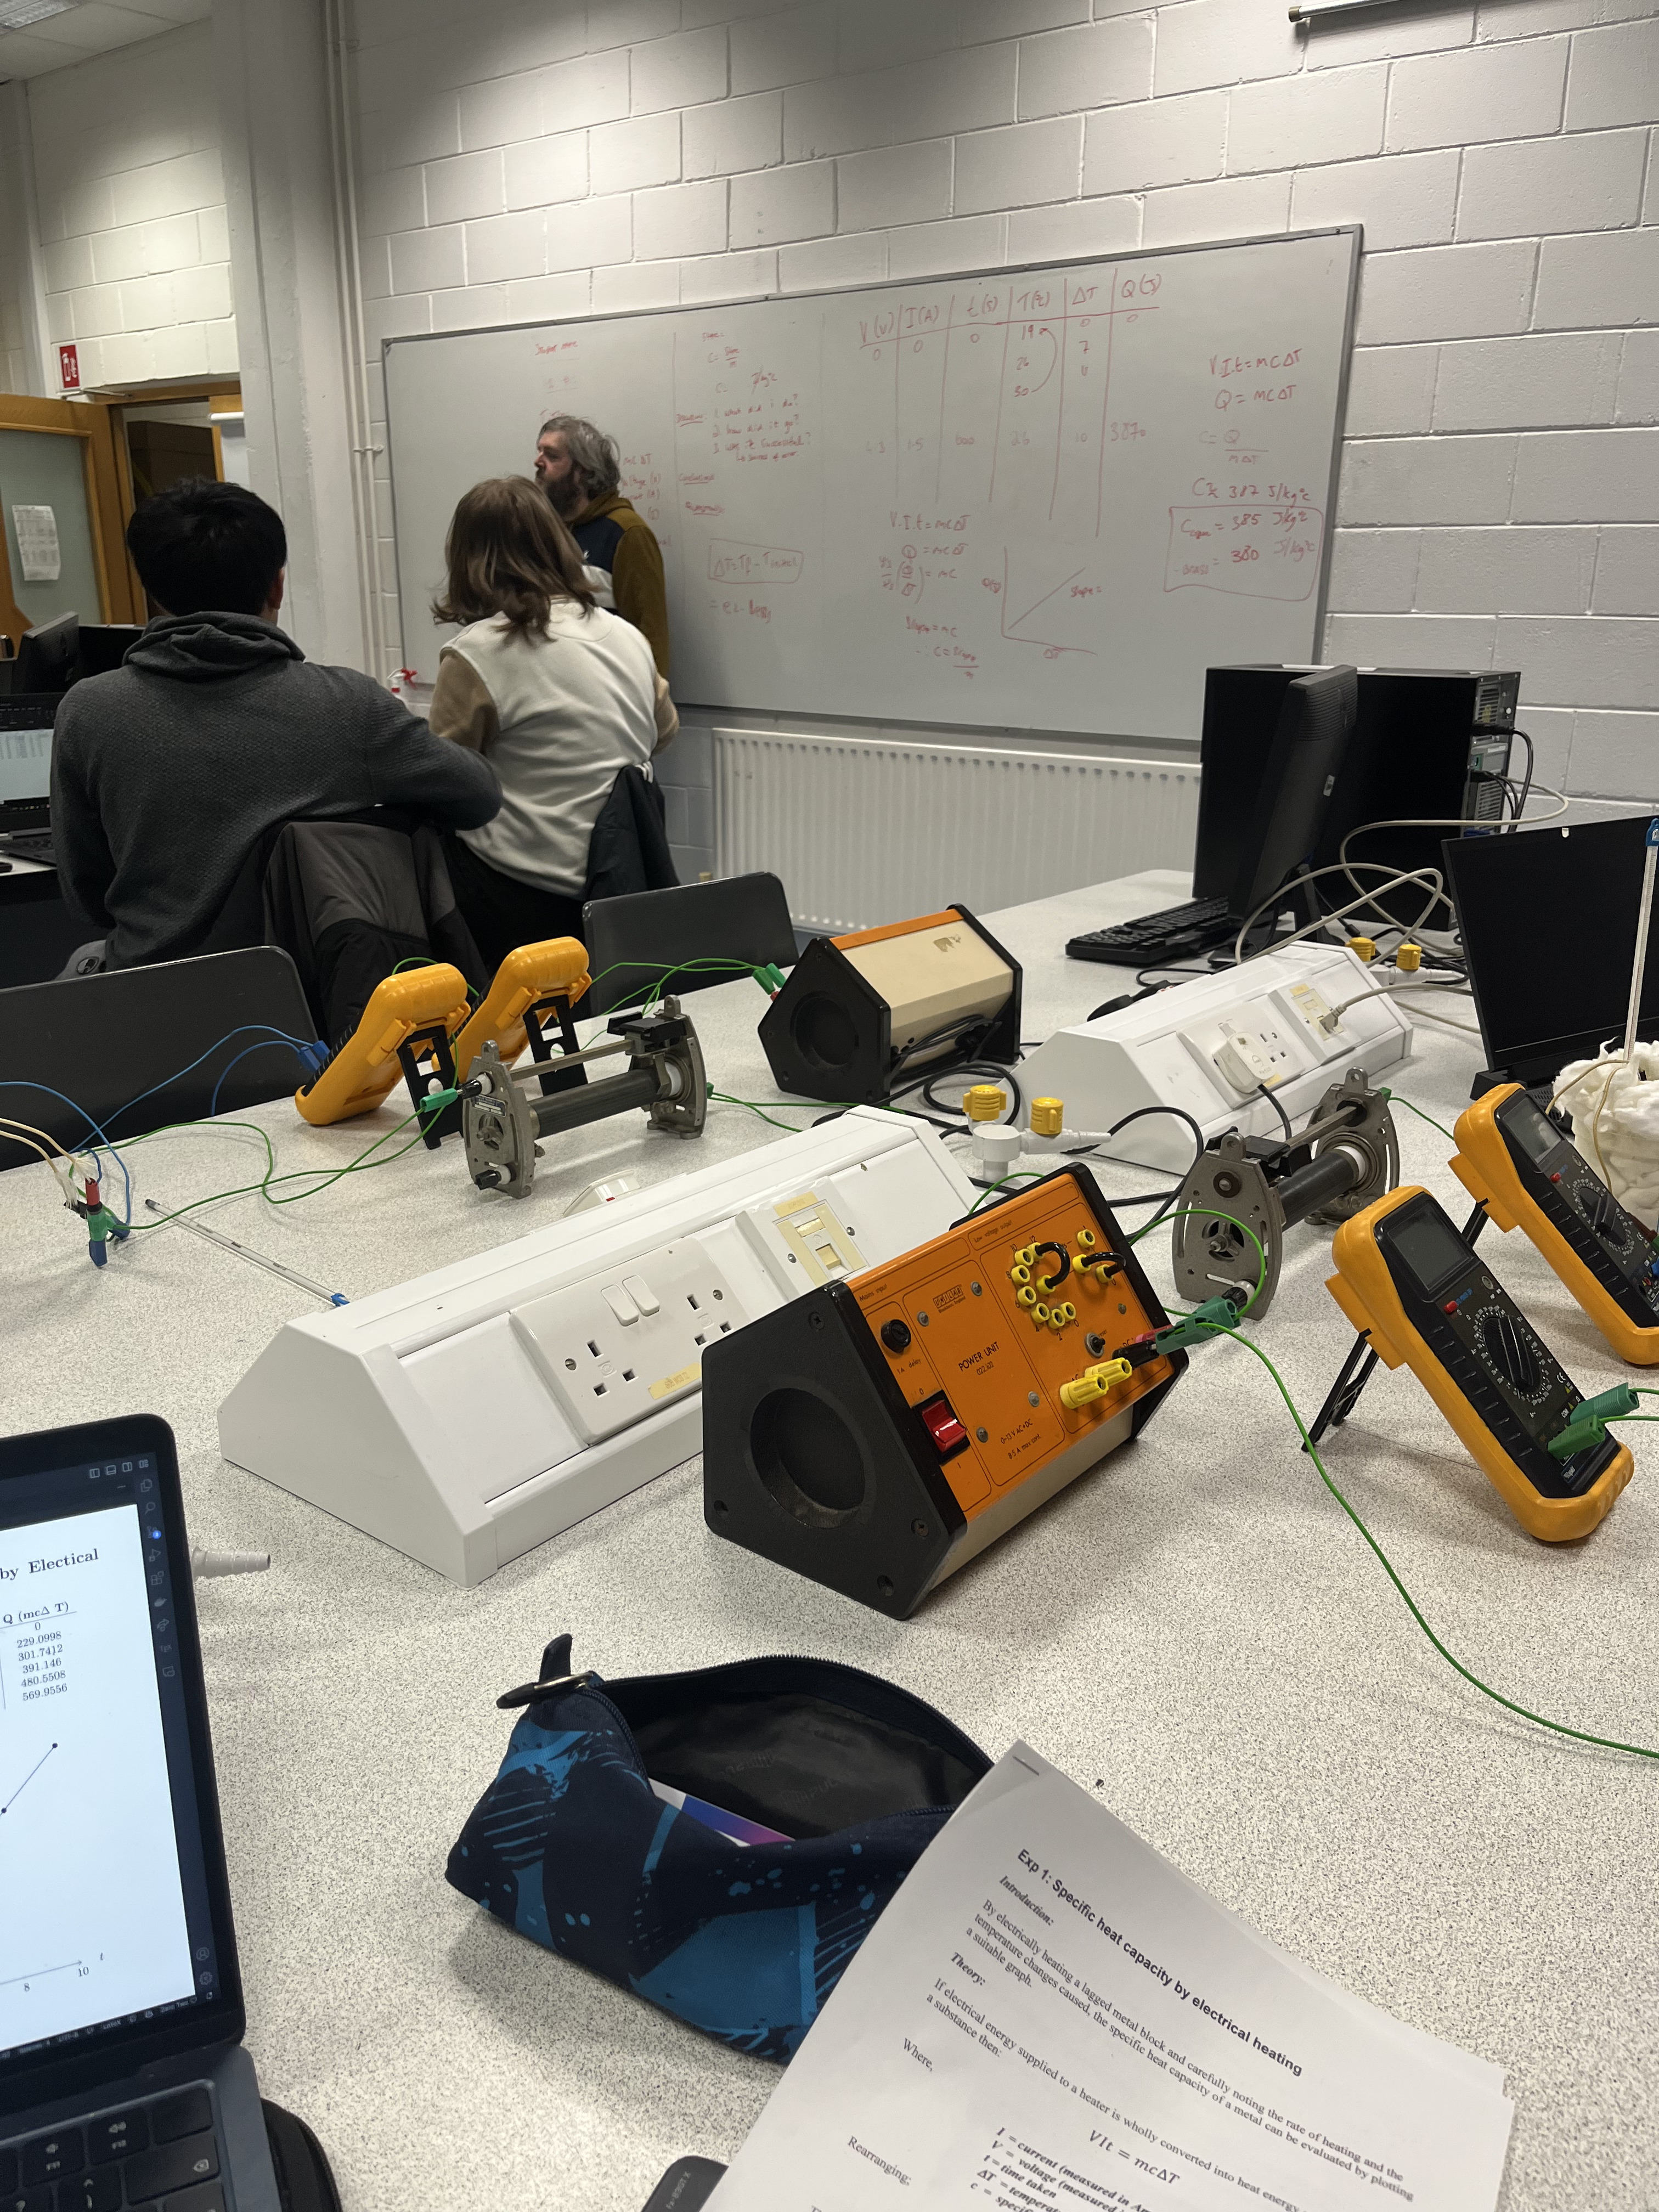
\includegraphics[width=0.6\textwidth]{IMG_5527.jpg}
\end{figure}


\subsection{Experiment}
\begin{figure}[H]
\centering
\begin{tabular}{c|c|c|c|c|c}
    \textbf{V (volt)} & \textbf{I (Ampere)} & \textbf{t (s)} & \textbf{Temp (°C)} & \textbf{$\Delta$ T} & \textbf{Q (mc$\Delta$ T)} \\
    \hline
    0 & 0 & 0 & 17 & 0 & 0\\
    8.34 & 2.7 & 120 & 20.5 & 3.5 & 2702.16\\
    8.34 & 2.7 & 240 & 27 & 10 & 5404.32\\
    8.34 & 2.7 & 360 & 35 & 18 & 8106 \\
    8.4 & 2.7 & 480 & 43 & 26 &  10808\\
    8.3 & 2.7 & 600 & 51 & 34 & 13510.8\\
\end{tabular}
\caption{Table of measurements}
\end{figure}



\begin{figure}[H]
    \centering
    \begin{tikzpicture}
        \begin{axis}[
            axis lines=middle,
            xlabel={$t$},
            ylabel={$\Delta T$},
            xtick={2,4,6,8,10},
            ytick={1,2,4,8,16,20, 30},
            ymin=0, ymax=35,
            xmin=0, xmax=10,
            axis line style={->},
            every axis x label/.style={
                at={(ticklabel* cs:1.05)},
                anchor=west,
            },
            every axis y label/.style={
                at={(ticklabel* cs:1.05)},
                anchor=south,
            }
        ]
        
    
        % Draw the plot and points
        \addplot[thick, mark=*] coordinates {(0,0) (2, 3.5) (4, 10) (6, 18) (8, 26) (10, 34)};
        
        \end{axis}
      \end{tikzpicture}
      \caption{Graph of $\Delta T$ against t}
    \end{figure}


    \begin{figure}[H]
        \centering
        \begin{tikzpicture}
            \begin{axis}[
                axis lines=middle,
                xlabel={$\Delta T$},
                ylabel={$Q$},
                xtick={5,10,15,20,25,30,35},
                ytick={0,1000,5000,10000,15000,20000},
                ymin=0, ymax=20000,
                xmin=0, xmax=40,
                axis line style={->},
                every axis x label/.style={
                    at={(ticklabel* cs:1.05)},
                    anchor=west,
                },
                every axis y label/.style={
                    at={(ticklabel* cs:1.05)},
                    anchor=south,
                }
            ]
            
        
            % Draw the plot and points
            \addplot[thick, mark=*] coordinates {(0, 0) (3.5, 2702.16) (10, 5404.32) (18, 8106) (26, 10808) (34, 13510.8)};
            
            \end{axis}
          \end{tikzpicture}
          \caption{Graph of Q against $\Delta T$}
        \end{figure}
    \subsection{Questions}
    \begin{enumerate}
        \item \textbf{In your opinion, is it important that the block is well insulated during the experiment? Why?}
        It is important since proper insulation ensures that most of 
        the electrical energy supplied to the block is used to increase its temperature rather than 
        being lost to the surroundings.
        \item \textbf{If you were to increase the current (A) used in this experiment, to a value higher than you used, would it change the experiment in any way? Give reasons as to your answer.}
        Uncreasing the current beyond 2.7 Ampere, would definitely change the experiment. The rate of heating would increase, and the temperature of the block would increase more rapidly. This would make it more difficult to measure the temperature accurately and to record the data in a timely manner.
        \item \textbf{What is the function of the big variable resistor (rheostat) in this experiment? Give reasons as to you answer.}
        The big variable resistor (rheostat) is used to control the current flowing through the circuit. By adjusting the resistance of the rheostat, the current can be adjusted to the desired value. This allows the rate of heating of the block to be controlled and the temperature changes to be measured accurately.
    \end{enumerate}

    \subsection{Conclusion}
    We found the slope coeffienct which 379,9975. We just divide the slope by the mass of the material to get the specific heat capacity of the material. The specific heat capacity of the material is 385 J/kg°C. Which exactly matches \textbf{the specific heat capacity of the material we were testing.}

\section{Exp 3 - Calibration of a Thermocouple, 11/02/2025}

\subsection{Theory}

A Thermocouple is formed by joining two metals. When two different metals are joined and connected through a sensitive voltmeter, it is found that whenever
a temperature difference exists between the junctions a reading is recorded on the voltmeter.
The greater the temperature difference between the junctions the larget the reading.
This property of the Thermocouple can be used to measure temperature. In practice the cold conjuction is maintained 
at a fix temperature i.e 0° C.

\subsubsection{Aim(s)}

The aim of the experiment is to calibrate a Thermocouple.

\subsubsection{Procedure}

As in lab manual.

\subsection{Diagrams/Apparaths}

Voltmeter, 2 Becker, Thermocouple, thermometer.

\begin{figure}[H]
    \centering
    \begin{tabular}{c|c|c|c|c|c}
        Temperature (°C) & Voltage (mV) Hot & Voltage (mV) Cold & Average Voltage (mV) \\ 
        \hline
        0 & 0 & 0 & 0\\
        10 & 0.1 & 0.35 & 0.05\\
        20 & 0.4 & 0.3 & 0.35\\
        30 & 1.1 & 0.9 & 1\\
        40 & 1.5 & 1.3 & 1.4\\
        50 & 2.1 & 1.6 & 1.7\\
        60 & 2.3 & 2.1 & 2.2\\
        70 & 2.7 & 2.4 & 2.55\\
        80 & 3 & 2.8 & 2.9\\
        90 & 3.5 & 3.2 & 3.35\\ 
        100 & 3.8 & 3.7 & 3.75\\
    \end{tabular}
    \caption{Table of measurements}
    \end{figure}

    \begin{figure}[H]
        \centering
        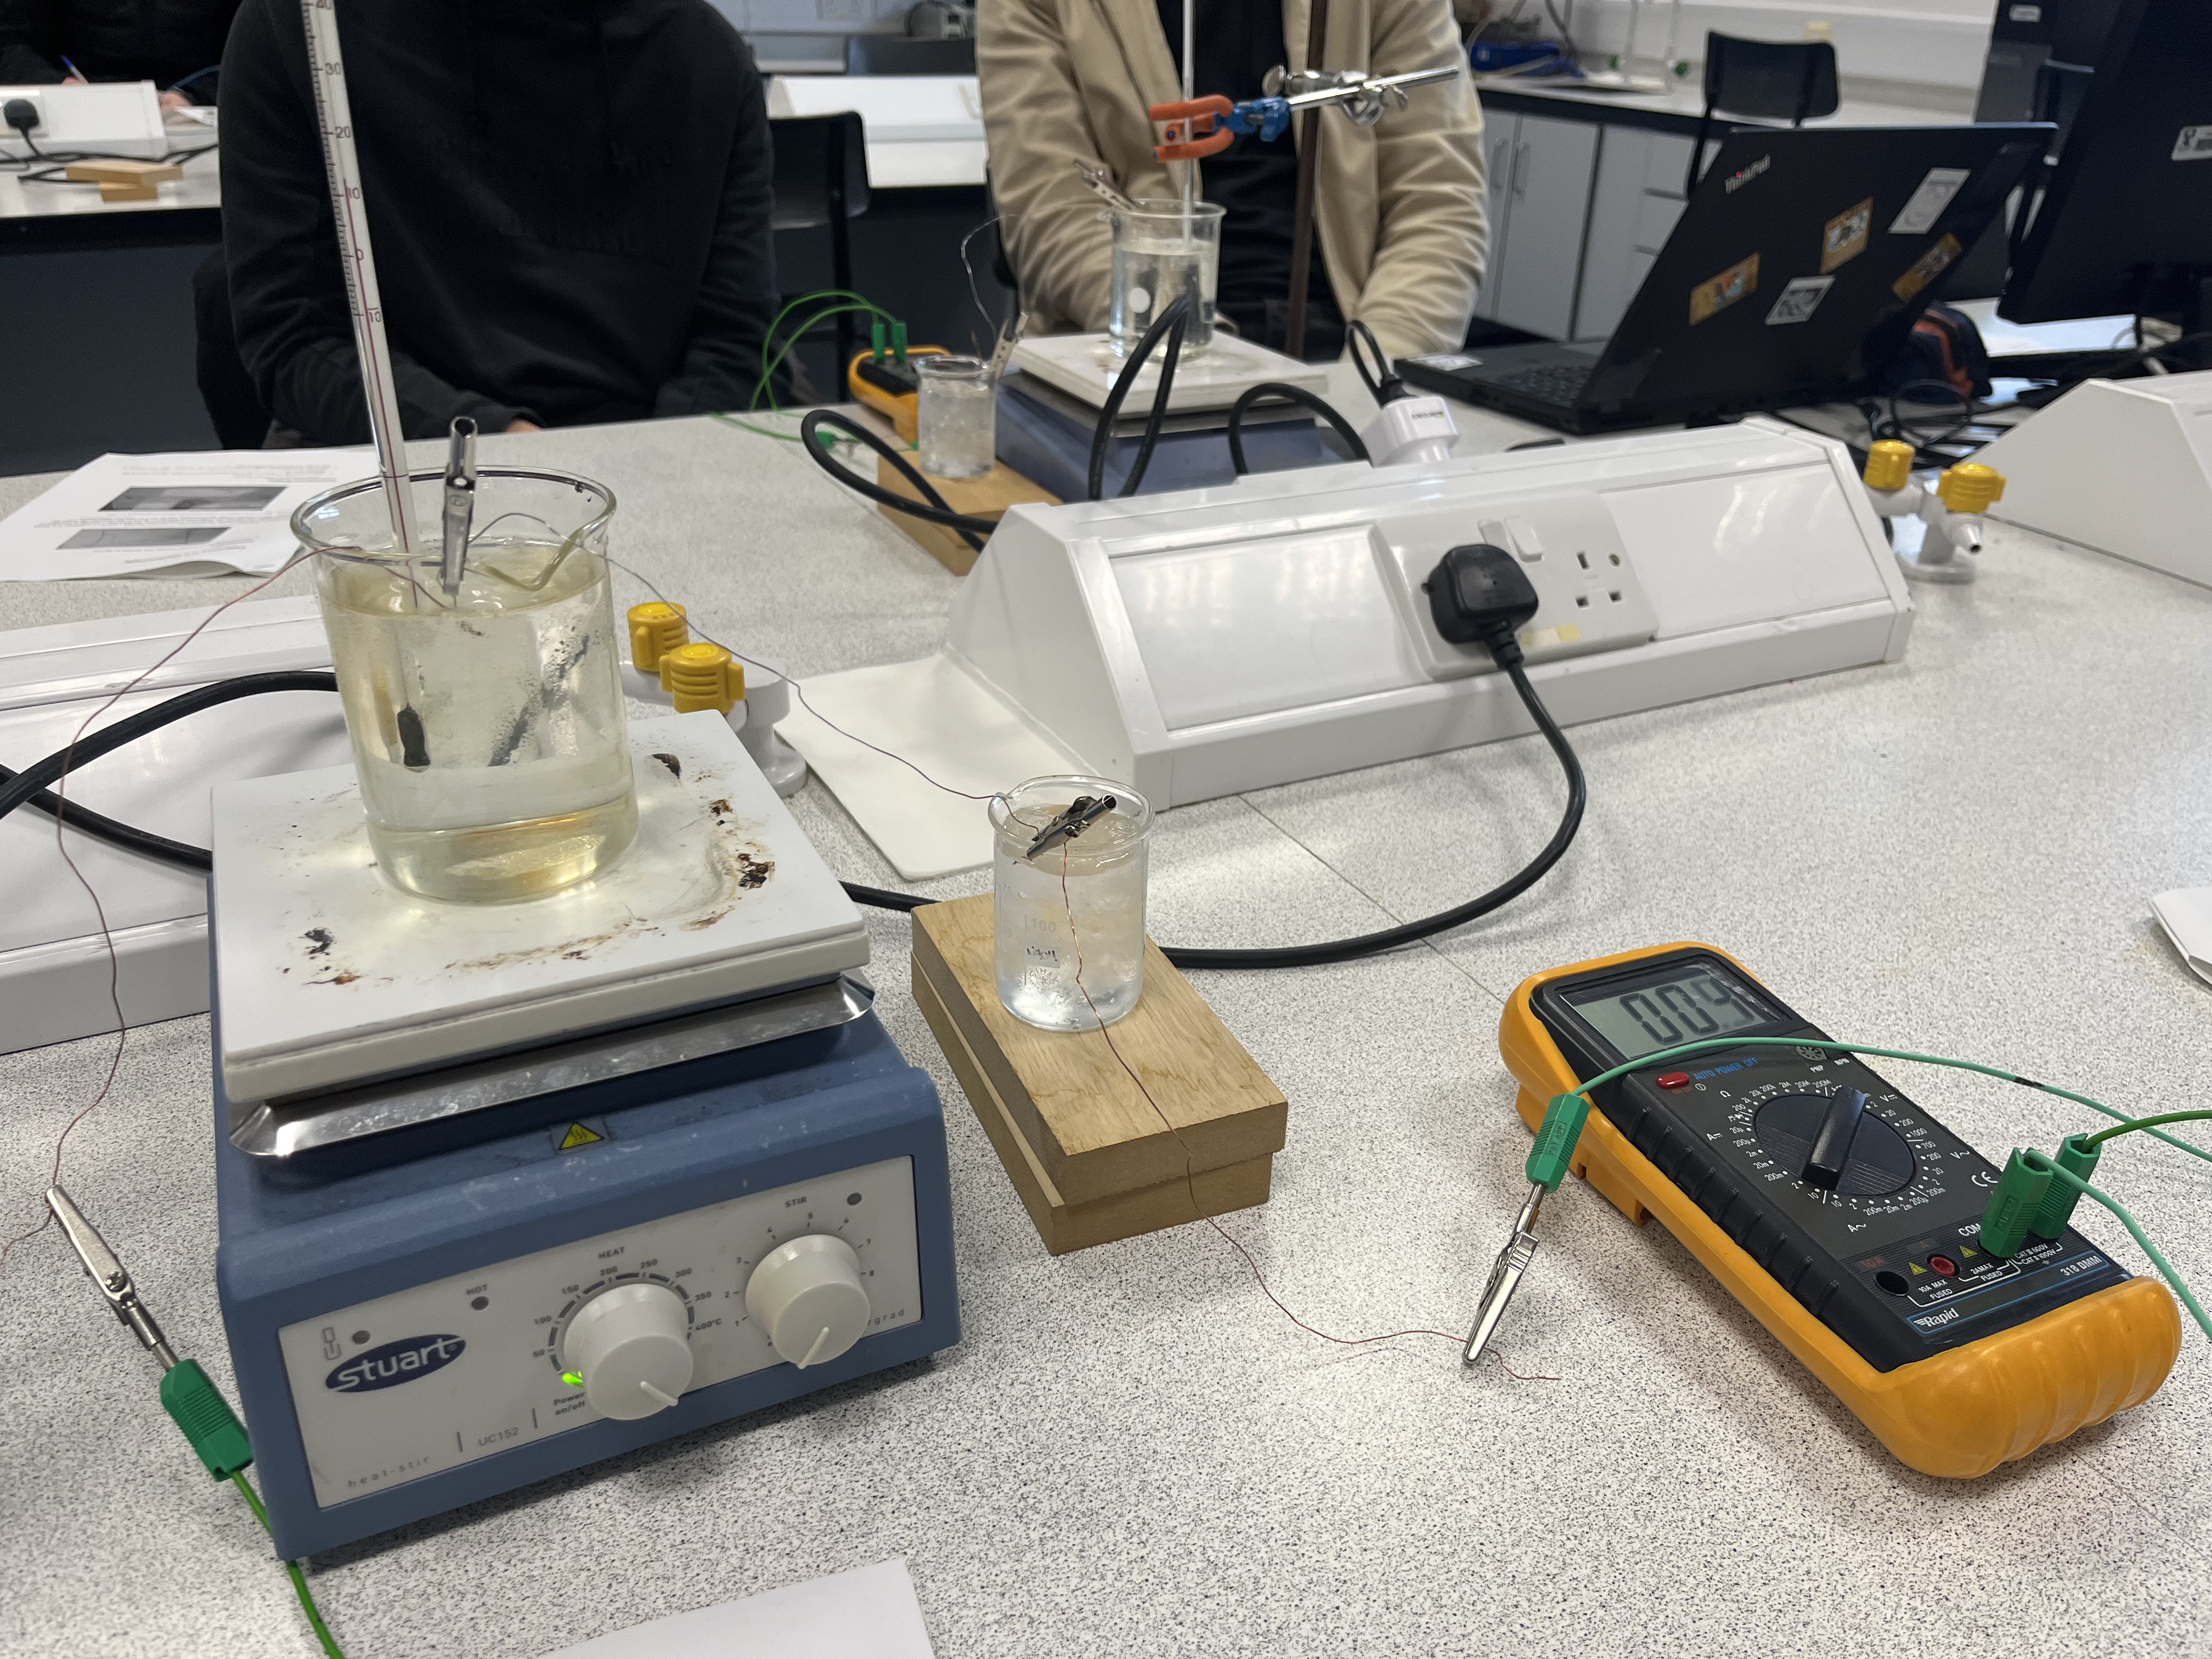
\includegraphics[width=1\textwidth]{IMG_5970.jpg}
        \label{fig:centered-image}
    \end{figure}

    \begin{figure}[H]
        \centering
        \begin{tikzpicture}
            \begin{axis}[
                axis lines=middle,
                xlabel={$t$},
                ylabel={$\Delta T$},
                xtick={10, 20, 30, 40, 50, 60, 70, 80, 90, 100},
                ytick={0, 0.5, 1, 1.5, 2, 2.5, 3, 3.5, 4},
                ymin=0, ymax=4,
                xmin=0, xmax=100,
                axis line style={->},
                every axis x label/.style={
                    at={(ticklabel* cs:1.05)},
                    anchor=west,
                },
                every axis y label/.style={
                    at={(ticklabel* cs:1.05)},
                    anchor=south,
                }
            ]
            
        
            % Draw the plot and points
            \addplot[thick, mark=*] coordinates {(0,0) (10, 0.05) (20, 0.35) (30, 1) (40, 1.4) (50, 1.7) (60, 2.2) (70, 2.55) (80, 2.9) (90, 3.35) (100, 3.75)};
            
            \end{axis}
          \end{tikzpicture}
          \caption{Graph of Average Voltage against Temperature}
        \end{figure}

        So we found that the equation for this graph is:
        \[y = 0.04x - 0.2114\]

\subsection{Questions}

Use the thermocouple and the calibration graph to estimate:

\begin{itemize}
    \item a. Room Temperature $\rightarrow$ 19°C so using the graph equation:  $y = 0.04x - 0.2114 \rightarrow 0.5486$ 
    \item b. Body Temperature $\rightarrow$ 37°C $\rightarrow (37 * 0.04) - 0.2114 = 1.2686$
    \item c. The temperature of water from the tap in the lab $\rightarrow 17.5$ °C $(17.5 * 0.04) - 0.2114 = 0,4886 $ 
\end{itemize}

\section{Exp 5 - RC Circuity}

\subsection{Theory}

It can be shown that the voltage and the current in the current in the circuit as follow:

\[V_c(t) = V_0 (1 - e^{-\frac{t}{\tau}})\]
\[I(t) = \frac{V_0}{R}e^{-\frac{t}{\tau}}\]
where $\tau = CR$.
In this experiment we are going to show these relationships.


\subsubsection{Aim(s)}

To build and test an RC circuit under (a) charge and (b) discharge conditions

\subsection{Experiment}

\subsubsection{Charging}

\begin{figure}[H]
\centering
\begin{tabular}{|c|c|}
    \hline
    Time (s) & Voltage (V)\\
    \hline
    0 & 0\\
    5 & 0.20\\
    10 & 0.45\\
    15 & 0.69\\
    20 & 1.1\\
    \vdots & \vdots\\
    60 & 2.65\\
    120 & 4.20\\
    180 & 5.45\\
    240 & 6.40\\
    300 & 7.12\\
    360 & 7.70\\
    420 & 8.14\\
    480 & 8.50\\
    540 & 8.83\\
    600 & 9.17\\
    \vdots & \vdots\\
    1380 & 9.99\\
    \hline   
\end{tabular}
\caption{Table of measurements while charging the circuits}
\end{figure}

\begin{figure}[H]
    \centering
    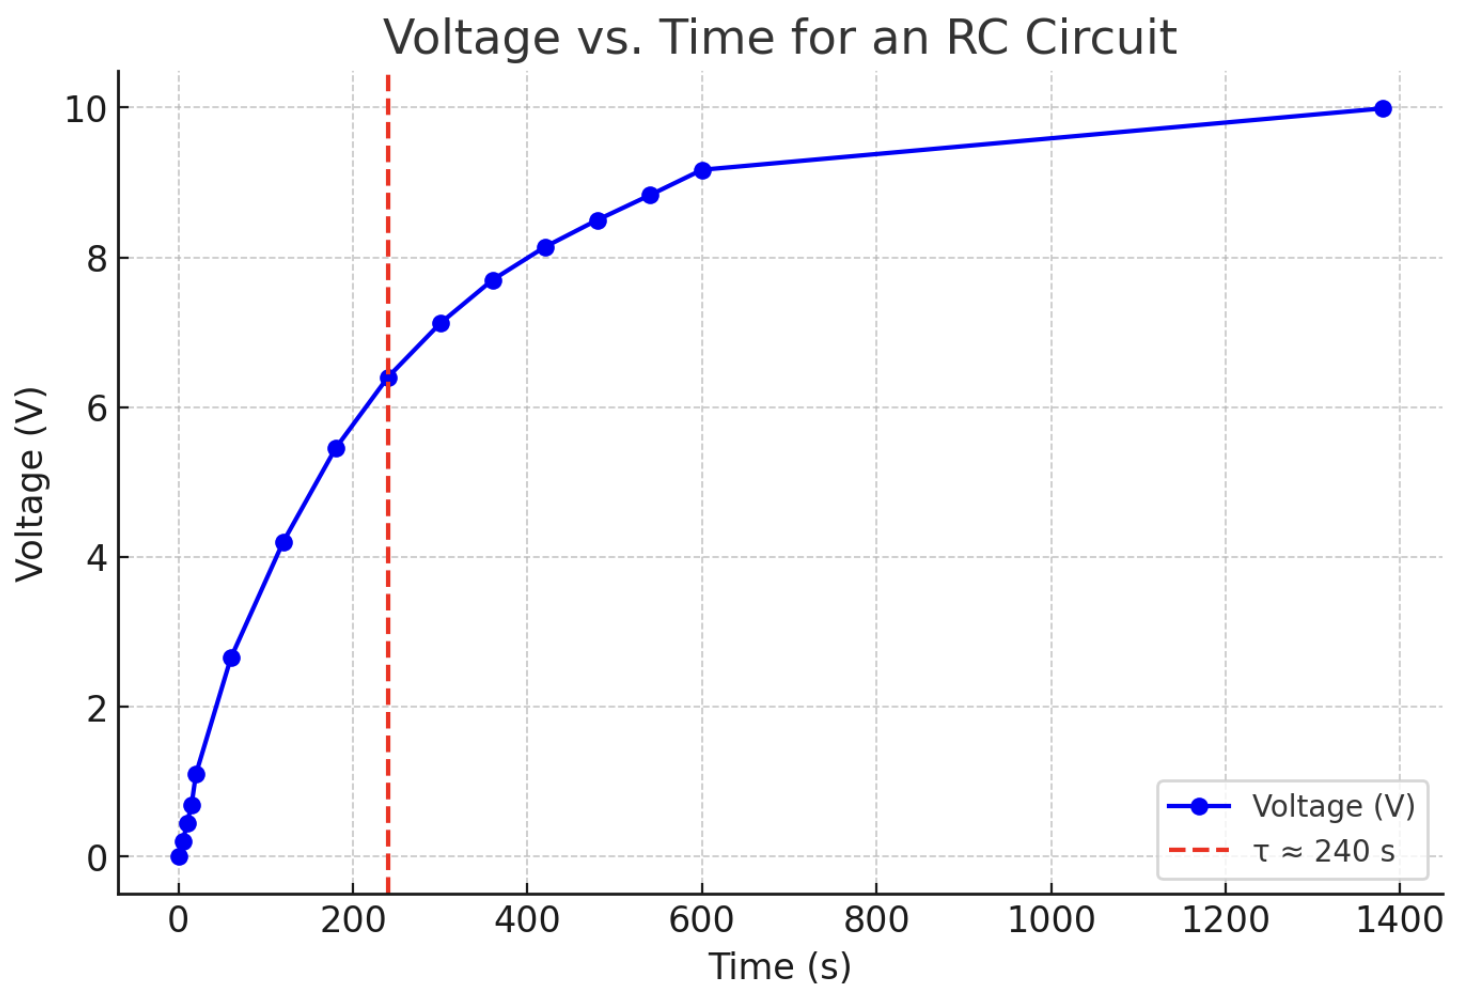
\includegraphics[width=1\textwidth]{Exp5.png}
    \caption{Graph of Voltage against Time}
\end{figure}
\noindent
The RC time constant ($\tau$) is estimated to be approximately 240 seconds, as indicated by 
the red dashed line at the time where the voltage reaches $63\%$ of its final value

\subsubsection{Discharging}

\begin{figure}[H]
    \centering
    \begin{tabular}{|c|c|}
        \hline
        Time (s) & Voltage (V)\\
        \hline
        0 & 10\\
        5 & 9.95\\
        10 & 9.92\\
        15 & 9.90\\
        20 & 9.87\\
        \vdots & \vdots\\
        60 & 9.65\\
        120 & 9.35\\
        180 & 9.10\\
        240 & 8.90\\
        300 & 8.70\\
        360 & 8.50\\
        420 & 8.30\\
        \vdots & \vdots\\
        A long time & 0.1\\
        \hline   
    \end{tabular}
\caption{Table of measurements while discharging the circuits}
\end{figure}

\begin{figure}[H]
    \centering
    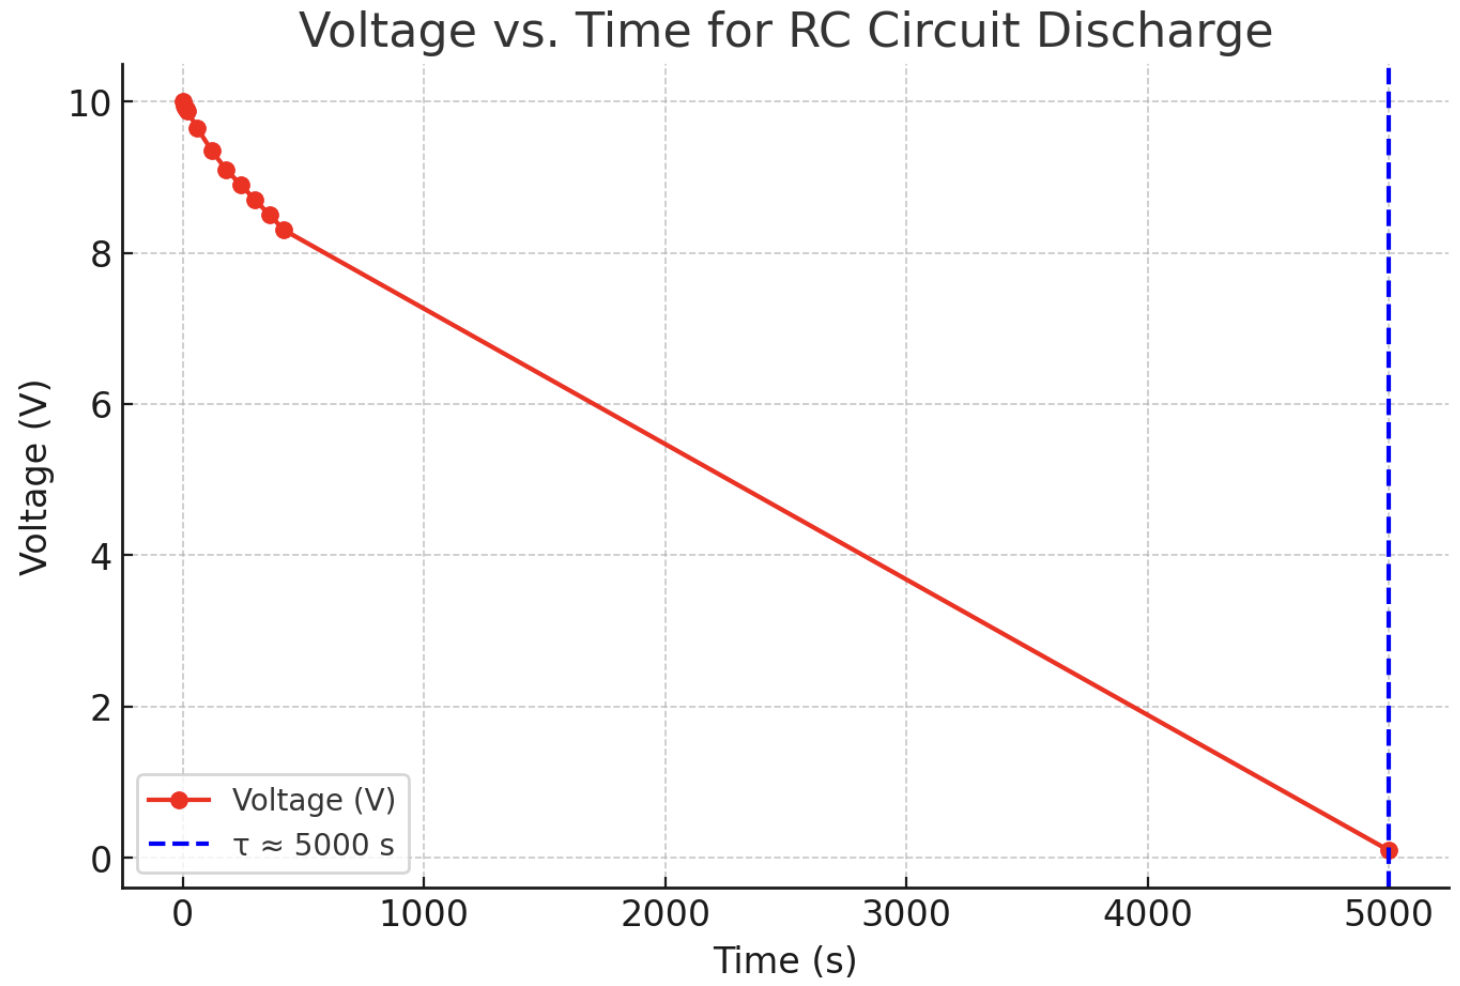
\includegraphics[width=1\textwidth]{Exp52.png}
    \caption{Graph of Voltage against Time while discharging}
\end{figure}
\noindent
The plot of Voltage (V) versus Time (s) for the discharging circuit shows an exponential decay. However, based on the extracted data, the estimated RC time constant ($\tau$) appears to be around 5000 seconds, which seems too large and might be due to the lack of a closer data point near $37\%$ of the initial voltage.
\\
\textbf{Questions:}
\begin{itemize}
    \item \textbf{Does the graph follow the expected shape for an RC circuit?} Yes, the graph follows the expected shape for an RC circuit which is an exponential decay for the discharging circuit and an exponential growth for the charging circuit.
    \item \textbf{What is the value of $\tau$, the time constant for your circuit?} We have that $R = 0.230 \times 10^6 \Omega$ and $C = 1000 \times 10^{-6} F$. The theoretical RC time constant $\tau$ is 230 seconds. This is close to our earlier estimated value of 240 seconds from the charging experiment, which suggests that our experimental data is reasonably accurate.
    \item \textbf{How does this compare to your experimental value? ($67.3\%$ of voltage in charge, $32.7\%$ of voltage in discharge).} The experimental value of the time constant for the charging circuit is close to the theoretical value, as the voltage reaches $63\%$ of its final value at 240 seconds. However, the time constant for the discharging circuit is significantly larger than the theoretical value, which might be due to the lack of a closer data point near $37\%$ of the initial voltage.
\end{itemize}


\section{Exp 5 - Experiments on Half-wave and Full-wave Rectifiers}

\subsection{Aim}

The objectives of this experiment are:

\begin{enumerate}
    \item To display a sinusoidal electrical signal on an oscilloscope and measure its amplitude and frequence
    \item To set up a halw-wave rectifier circuit and investigate its operation using the oscilloscope
    \item To set up a full-wave rectifier circuit and investigate its operation using the oscilloscope
\end{enumerate}

An AC signal when passed through a half wave rectifier will yield the following action:

\begin{figure}[H]
    \centering
    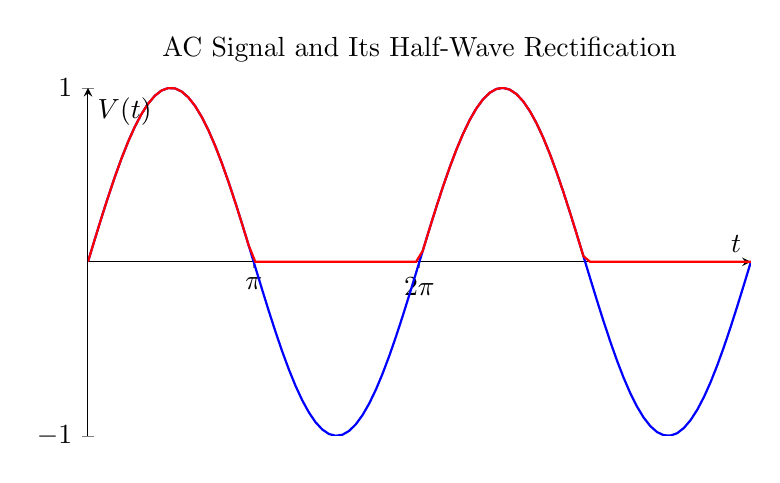
\begin{tikzpicture}
        \begin{axis}[
            domain=0:4*pi,
            samples=100,
            xlabel={$t$},
            ylabel={$V(t)$},
            axis lines=middle,
            legend pos=south east,
            legend style={font=\large},
            width=10cm,
            height=6cm,
            xtick={0,pi,2*pi},
            xticklabels={$0$,$\pi$,$2\pi$},
            ytick={-1,0,1},
            yticklabels={$-1$,$0$,$1$},
            title={AC Signal and Its Half-Wave Rectification}
          ]
          % Plot of the original AC signal: V_in(t) = sin(t)
          \addplot[blue, thick] {sin(deg(x))};
          % Plot of the half-wave rectified signal: V_out(t) = sin(t) for sin(t)>=0, 0 otherwise.
          \addplot[red, thick, domain=0:4*pi] { (sin(deg(x))>0) ? sin(deg(x)) : 0 };
        \end{axis}
      \end{tikzpicture}
\end{figure}
and so the function displays as follows:
\[V_{out}(t)=\begin{cases}\sin(t)&\text{if }\sin(t)\ge0\\0&\text{if }\sin(t)<0\end{cases}\]


Whereas, a full-wave rectifier would yield the following action:

\begin{figure}[H]
    \centering
    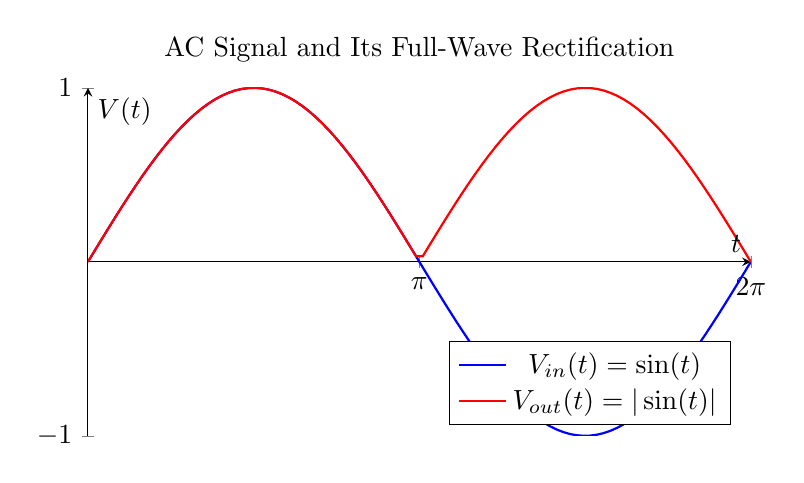
\begin{tikzpicture}
        \begin{axis}[
            domain=0:2*pi,
            samples=100,
            xlabel={$t$},
            ylabel={$V(t)$},
            axis lines=middle,
            legend pos=south east,
            width=10cm, height=6cm,
            xtick={0,pi,2*pi},
            xticklabels={$0$,$\pi$,$2\pi$},
            ytick={-1, 0, 1},
            yticklabels={$-1$,$0$,$1$},
            title={AC Signal and Its Full-Wave Rectification}
          ]
          % Plot of the original AC signal: V_in(t) = sin(t)
          \addplot[blue, thick] {sin(deg(x))};
          \addlegendentry{$V_{in}(t) = \sin(t)$};
          
          % Plot of the rectified signal: V_out(t) = |sin(t)|
          \addplot[red, thick] {abs(sin(deg(x)))};
          \addlegendentry{$V_{out}(t) = |\sin(t)|$};
        \end{axis}
      \end{tikzpicture}

\end{figure}
\noindent
This signal may also be further smoothed using a capacitor on the output.


\subsection{Procedure}

As in lab manual.

\subsection{Tools}

\begin{itemize}
    \item Oscilloscope
    \item Breadboard
    \item Resistor (1 k$\Omega$)
    \item Diode 
    \item AC Power Supply
\end{itemize}

\subsection{Determing the frequency of the AC Power Supply}

\begin{itemize}
    \item Set the AC Power supply to output an AC Voltage of 5 volts.
    \item Connect an appropriate lead to CH-1 of the oscilloscope.
    \item Connect the croc-clip of the coaxial cable across the resistor in the circuit.
    \item We measured: 24 volts for \textbf{peak-to-peak voltage} and 50 Hz for \textbf{frequency}. The peak amplitude was 12 volts.
    \[Volts/Div = 5v \; \; \; \; \; Time/Div = 10ms\]
\end{itemize}

\begin{figure}[H]
    \centering
    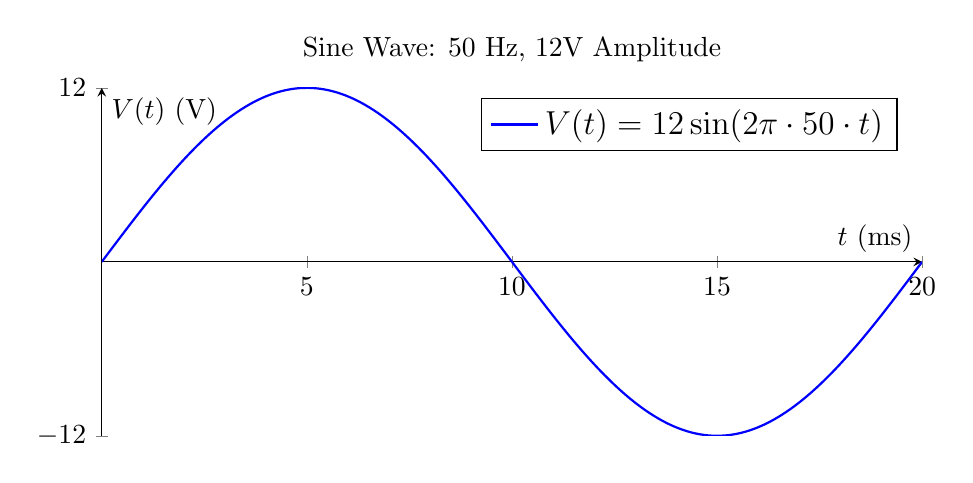
\begin{tikzpicture}
        \begin{axis}[
            domain=0:20, % Time in milliseconds
            samples=200,
            xlabel={$t$ (ms)},
            ylabel={$V(t)$ (V)},
            axis lines=middle,
            legend pos=north east,
            legend style={font=\large},
            width=12cm,
            height=6cm,
            xtick={0,5,10,15,20},
            xticklabels={$0$,$5$,$10$,$15$,$20$},
            ytick={-12, 0, 12},
            yticklabels={$-12$,$0$,$12$},
            title={Sine Wave: 50 Hz, 12V Amplitude}
          ]
          % Plot of the sine wave: V(t) = 12 sin(2π(50)t)
          \addplot[blue, thick] {12 * sin(deg(2 * pi * 50 * x / 1000))};
          \addlegendentry{$V(t) = 12 \sin(2\pi \cdot 50 \cdot t)$};
        \end{axis}
      \end{tikzpicture}
\end{figure}

\subsection{Half-wave rectifier}

\begin{itemize}
    \item Modify the circuit to include a half-wave rectifier.
    \item Set the AC Power supply to output an AC Voltage of 5 volts.
    \item Connect an appropriate lead to CH-1 of the oscilloscope.
    \item Connect the croc-clip of the coaxial cable across the resistor in the circuit.
    \item We measured: 6.40 volts for \textbf{peak voltage} and 49.80 Hz for \textbf{frequency}.
    \[Volts/Div = 2v \; \; \; \; \; Time/Div = 10ms\]
\end{itemize}

\begin{figure}[H]
    \centering
    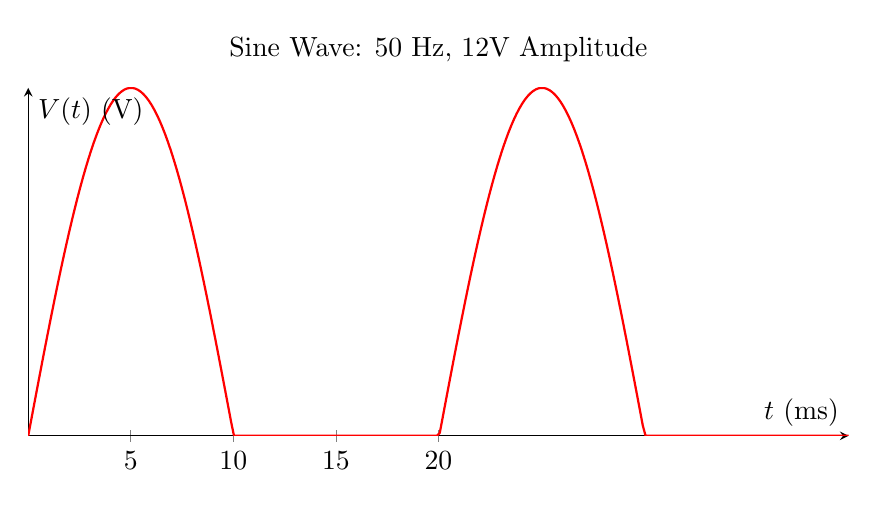
\begin{tikzpicture}
        \begin{axis}[
            domain=0:40, % Time in milliseconds
            samples=300,
            xlabel={$t$ (ms)},
            ylabel={$V(t)$ (V)},
            axis lines=middle,
            legend pos=north east,
            legend style={font=\large},
            width=12cm,
            height=6cm,
            xtick={0,5,10,15,20},
            xticklabels={$0$,$5$,$10$,$15$,$20$},
            ytick={-12, 0, 12},
            yticklabels={$-12$,$0$,$12$},
            title={Sine Wave: 50 Hz, 12V Amplitude}
          ]
          % Plot of the sine wave: V(t) = 12 sin(2π(50)t)
          \addplot[red, thick] { 6.40 * sin(deg(2 * pi * 49.90 * x / 1000))>0 ? 6.40 * sin(deg(2 * pi * 49.90 * x / 1000)) : 0 };
        \end{axis}
      \end{tikzpicture}
\end{figure}

\subsection{Full-wave rectifier}

\begin{itemize}
    \item Modify the circuits to include a full-wave rectifier.
    \item Set the AC Power supply to output an AC Voltage of 5 volts.
    \item Connect an appropriate lead to CH-1 of the oscilloscope.
    \item Connect the croc-clip of the coaxial cable across the resistor in the circuit.
    \item We measured: 2.56 volts for \textbf{peak voltage} and 100 Hz for \textbf{frequency}. 
    \[Volts/Div = 2v \; \; \; \; \; Time/Div = 10ms\]
\end{itemize}

\begin{figure}[H]
    \centering
    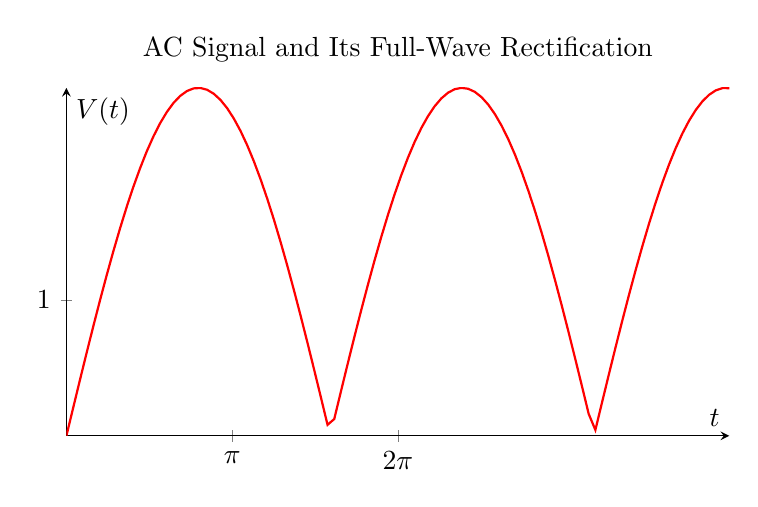
\begin{tikzpicture}
        \begin{axis}[
            domain=0:4*pi,
            samples=100,
            xlabel={$t$},
            ylabel={$V(t)$},
            axis lines=middle,
            legend pos=south east,
            width=10cm, height=6cm,
            xtick={0,pi,2*pi},
            xticklabels={$0$,$\pi$,$2\pi$},
            ytick={-1, 0, 1},
            yticklabels={$-1$,$0$,$1$},
            title={AC Signal and Its Full-Wave Rectification}
          ]
          
          % Plot of the rectified signal: V_out(t) = |sin(t)|
          \addplot[red, thick] {abs(2.56 * sin(deg(2 * pi * 100 * x / 1000)))};
        \end{axis}
      \end{tikzpicture}

\end{figure}

\subsection{Questions}

\begin{enumerate}
    \item \textbf{What are the main sources of error in this experiment?} The main sources of error in this experiment could be due to the accuracy of the oscilloscope measurements, the precision of the resistor values, and any noise or interference in the AC power supply.
    \item \textbf{What features of the oscilloscope make it an extremely useful form of voltmeter?} The oscilloscope is extremely useful because it can display the waveform of the voltage signal in real-time, allowing for the measurement of both the amplitude and frequency of the signal. 
    \item \textbf{Explain how you would determine the rms value of an ac signal using the oscilloscope.} To determine the rms value of an AC signal using the oscilloscope, you would measure the peak voltage (Vp) and then calculate the rms value using the formula:
    \[V_{rms} = \frac{V_{pp}}{\sqrt{2}}\]
    Sometimes the oscilloscope has a built-in function to directly measure the rms value of the AC signal.
\end{enumerate}


\end{document}